\documentclass{standalone}
\usepackage{tikz}
\usetikzlibrary{patterns, positioning}
\usepackage[sfdefault]{ClearSans} %% option 'sfdefault' activates Clear Sans as the default text font
\usepackage[T1]{fontenc}

\begin{document}
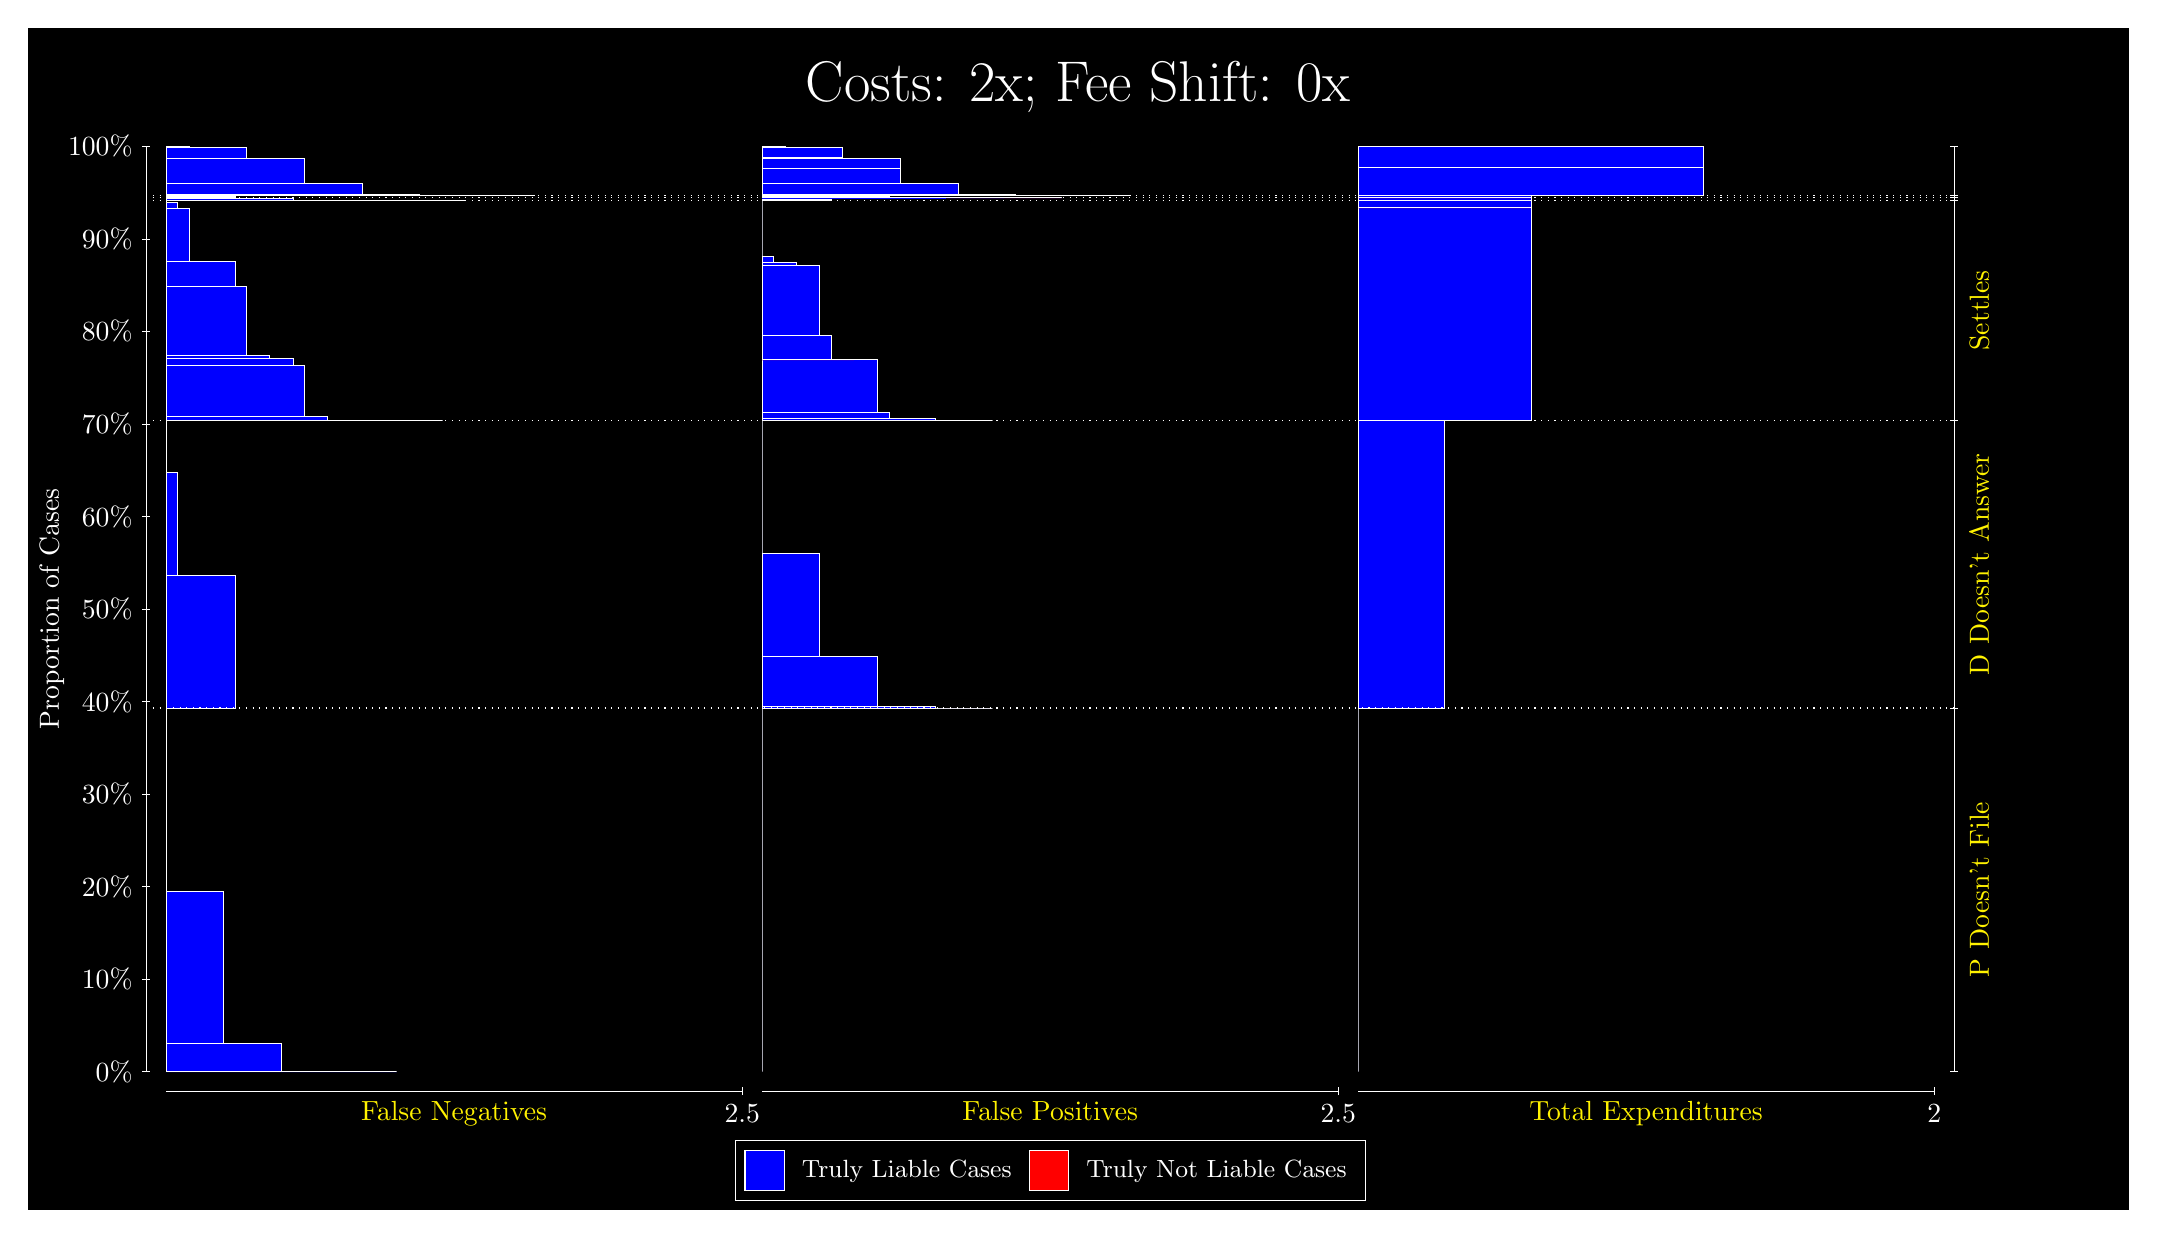
\begin{tikzpicture}
\draw[fill=black] (0,0) rectangle (26.667,15);
\draw[text=white] (0,13.5) rectangle (26.667,15) node[midway] {\huge Costs: 2x; Fee Shift: 0x};
\draw[white, very thin] (1.5,1.75) -- (1.5,13.5);
\node[rotate=90, text=white, anchor=center] at (0.3, 7.625) {Proportion of Cases};
\draw[white, very thin] (1.45,1.75) -- (1.55,1.75);
\node[text=white, anchor=east] at (1.45, 1.75) {0\%};
\draw[white, very thin] (1.45,2.925) -- (1.55,2.925);
\node[text=white, anchor=east] at (1.45, 2.925) {10\%};
\draw[white, very thin] (1.45,4.1) -- (1.55,4.1);
\node[text=white, anchor=east] at (1.45, 4.1) {20\%};
\draw[white, very thin] (1.45,5.275) -- (1.55,5.275);
\node[text=white, anchor=east] at (1.45, 5.275) {30\%};
\draw[white, very thin] (1.45,6.45) -- (1.55,6.45);
\node[text=white, anchor=east] at (1.45, 6.45) {40\%};
\draw[white, very thin] (1.45,7.625) -- (1.55,7.625);
\node[text=white, anchor=east] at (1.45, 7.625) {50\%};
\draw[white, very thin] (1.45,8.8) -- (1.55,8.8);
\node[text=white, anchor=east] at (1.45, 8.8) {60\%};
\draw[white, very thin] (1.45,9.975) -- (1.55,9.975);
\node[text=white, anchor=east] at (1.45, 9.975) {70\%};
\draw[white, very thin] (1.45,11.15) -- (1.55,11.15);
\node[text=white, anchor=east] at (1.45, 11.15) {80\%};
\draw[white, very thin] (1.45,12.325) -- (1.55,12.325);
\node[text=white, anchor=east] at (1.45, 12.325) {90\%};
\draw[white, very thin] (1.45,13.5) -- (1.55,13.5);
\node[text=white, anchor=east] at (1.45, 13.5) {100\%};

\draw[white, very thin] (24.457,1.75) -- (24.457,13.5);
\draw[white, very thin] (24.407,1.75) -- (24.507,1.75);
\node[anchor=west] at (24.407, 1.75) {};
\draw[white, very thin] (24.407,6.3668) -- (24.507,6.3668);
\node[anchor=west] at (24.407, 6.3668) {};
\draw[white, very thin] (24.407,10.02) -- (24.507,10.02);
\node[anchor=west] at (24.407, 10.02) {};
\draw[white, very thin] (24.407,12.814) -- (24.507,12.814);
\node[anchor=west] at (24.407, 12.814) {};
\draw[white, very thin] (24.407,12.848) -- (24.507,12.848);
\node[anchor=west] at (24.407, 12.848) {};
\draw[white, very thin] (24.407,12.88) -- (24.507,12.88);
\node[anchor=west] at (24.407, 12.88) {};
\draw[white, very thin] (24.407,13.5) -- (24.507,13.5);
\node[anchor=west] at (24.407, 13.5) {};

\draw[white, very thin, fill=blue] (1.75,1.75) rectangle (4.6775,1.75);
\draw[white, very thin, fill=blue] (1.75,1.75) rectangle (3.9457,1.7531);
\draw[white, very thin, fill=blue] (1.75,1.7531) rectangle (3.2138,2.1134);
\draw[white, very thin, fill=blue] (1.75,2.1134) rectangle (2.4819,4.0355);
\draw[white, very thin, fill=red] (1.75,4.0355) rectangle (1.75,4.0355);
\draw[white, very thin, fill=blue] (1.75,4.0355) rectangle (1.75,6.3668);
\draw[white, very thin, fill=blue] (1.75,6.3668) rectangle (2.6283,8.0505);
\draw[white, very thin, fill=blue] (1.75,8.0505) rectangle (1.8964,9.3624);
\draw[white, very thin, fill=red] (1.75,9.3624) rectangle (1.75,9.3624);
\draw[white, very thin, fill=blue] (1.75,9.3624) rectangle (1.75,10.02);
\draw[white, very thin, fill=blue] (1.75,10.02) rectangle (5.2631,10.02);
\draw[white, very thin, fill=blue] (1.75,10.02) rectangle (4.5312,10.021);
\draw[white, very thin, fill=blue] (1.75,10.021) rectangle (4.092,10.023);
\draw[white, very thin, fill=blue] (1.75,10.023) rectangle (3.7993,10.073);
\draw[white, very thin, fill=blue] (1.75,10.073) rectangle (3.5065,10.724);
\draw[white, very thin, fill=blue] (1.75,10.724) rectangle (3.3602,10.808);
\draw[white, very thin, fill=blue] (1.75,10.808) rectangle (3.0674,10.846);
\draw[white, very thin, fill=blue] (1.75,10.846) rectangle (2.7746,11.728);
\draw[white, very thin, fill=blue] (1.75,11.728) rectangle (2.6283,12.043);
\draw[white, very thin, fill=blue] (1.75,12.043) rectangle (2.3355,12.044);
\draw[white, very thin, fill=blue] (1.75,12.044) rectangle (2.0428,12.709);
\draw[white, very thin, fill=blue] (1.75,12.709) rectangle (1.8964,12.788);
\draw[white, very thin, fill=red] (1.75,12.788) rectangle (1.75,12.788);
\draw[white, very thin, fill=blue] (1.75,12.788) rectangle (1.75,12.814);
\draw[white, very thin, fill=blue] (1.75,12.814) rectangle (5.5558,12.814);
\draw[white, very thin, fill=blue] (1.75,12.814) rectangle (4.8239,12.814);
\draw[white, very thin, fill=blue] (1.75,12.814) rectangle (4.092,12.814);
\draw[white, very thin, fill=blue] (1.75,12.814) rectangle (3.3602,12.835);
\draw[white, very thin, fill=blue] (1.75,12.835) rectangle (2.6283,12.848);
\draw[white, very thin, fill=red] (1.75,12.848) rectangle (1.75,12.848);
\draw[white, very thin, fill=blue] (1.75,12.848) rectangle (2.6283,12.861);
\draw[white, very thin, fill=blue] (1.75,12.861) rectangle (1.8964,12.88);
\draw[white, very thin, fill=red] (1.75,12.88) rectangle (1.75,12.88);
\draw[white, very thin, fill=blue] (1.75,12.88) rectangle (1.75,12.88);
\draw[white, very thin, fill=blue] (1.75,12.88) rectangle (6.4341,12.88);
\draw[white, very thin, fill=blue] (1.75,12.88) rectangle (5.7022,12.88);
\draw[white, very thin, fill=blue] (1.75,12.88) rectangle (4.9703,12.888);
\draw[white, very thin, fill=blue] (1.75,12.888) rectangle (4.2384,13.032);
\draw[white, very thin, fill=blue] (1.75,13.032) rectangle (3.5065,13.343);
\draw[white, very thin, fill=blue] (1.75,13.343) rectangle (2.7746,13.487);
\draw[white, very thin, fill=blue] (1.75,13.487) rectangle (2.0428,13.5);
\draw[white, very thin, fill=red] (1.75,13.5) rectangle (1.75,13.5);
\draw[white, very thin, fill=blue] (1.75,13.5) rectangle (1.75,13.5);
\draw[white, very thin, fill=red] (9.3189,1.75) rectangle (9.3189,1.75);
\draw[white, very thin, fill=blue] (9.3189,1.75) rectangle (9.3189,6.3668);
\draw[white, very thin, fill=red] (9.3189,6.3668) rectangle (12.246,6.3668);
\draw[white, very thin, fill=blue] (9.3189,6.3668) rectangle (12.246,6.3668);
\draw[white, very thin, fill=blue] (9.3189,6.3668) rectangle (11.515,6.387);
\draw[white, very thin, fill=blue] (9.3189,6.387) rectangle (10.783,7.024);
\draw[white, very thin, fill=blue] (9.3189,7.024) rectangle (10.051,8.3359);
\draw[white, very thin, fill=blue] (9.3189,8.3359) rectangle (9.3189,10.02);
\draw[white, very thin, fill=red] (9.3189,10.02) rectangle (12.246,10.02);
\draw[white, very thin, fill=blue] (9.3189,10.02) rectangle (12.246,10.02);
\draw[white, very thin, fill=red] (9.3189,10.02) rectangle (11.661,10.02);
\draw[white, very thin, fill=blue] (9.3189,10.02) rectangle (11.661,10.022);
\draw[white, very thin, fill=blue] (9.3189,10.022) rectangle (11.515,10.045);
\draw[white, very thin, fill=blue] (9.3189,10.045) rectangle (10.929,10.125);
\draw[white, very thin, fill=blue] (9.3189,10.125) rectangle (10.783,10.79);
\draw[white, very thin, fill=red] (9.3189,10.79) rectangle (10.49,10.79);
\draw[white, very thin, fill=blue] (9.3189,10.79) rectangle (10.49,10.79);
\draw[white, very thin, fill=blue] (9.3189,10.79) rectangle (10.197,11.106);
\draw[white, very thin, fill=blue] (9.3189,11.106) rectangle (10.051,11.987);
\draw[white, very thin, fill=blue] (9.3189,11.987) rectangle (9.758,12.025);
\draw[white, very thin, fill=blue] (9.3189,12.025) rectangle (9.4652,12.109);
\draw[white, very thin, fill=blue] (9.3189,12.109) rectangle (9.3189,12.814);
\draw[white, very thin, fill=red] (9.3189,12.814) rectangle (10.197,12.814);
\draw[white, very thin, fill=blue] (9.3189,12.814) rectangle (10.197,12.827);
\draw[white, very thin, fill=blue] (9.3189,12.827) rectangle (9.4652,12.848);
\draw[white, very thin, fill=blue] (9.3189,12.848) rectangle (9.3189,12.848);
\draw[white, very thin, fill=red] (9.3189,12.848) rectangle (13.125,12.848);
\draw[white, very thin, fill=blue] (9.3189,12.848) rectangle (13.125,12.848);
\draw[white, very thin, fill=blue] (9.3189,12.848) rectangle (12.393,12.848);
\draw[white, very thin, fill=blue] (9.3189,12.848) rectangle (11.661,12.849);
\draw[white, very thin, fill=blue] (9.3189,12.849) rectangle (10.929,12.867);
\draw[white, very thin, fill=blue] (9.3189,12.867) rectangle (10.197,12.88);
\draw[white, very thin, fill=red] (9.3189,12.88) rectangle (14.003,12.88);
\draw[white, very thin, fill=blue] (9.3189,12.88) rectangle (14.003,12.88);
\draw[white, very thin, fill=red] (9.3189,12.88) rectangle (13.271,12.88);
\draw[white, very thin, fill=blue] (9.3189,12.88) rectangle (13.271,12.88);
\draw[white, very thin, fill=red] (9.3189,12.88) rectangle (12.539,12.88);
\draw[white, very thin, fill=blue] (9.3189,12.88) rectangle (12.539,12.893);
\draw[white, very thin, fill=blue] (9.3189,12.893) rectangle (11.807,13.036);
\draw[white, very thin, fill=red] (9.3189,13.036) rectangle (11.807,13.036);
\draw[white, very thin, fill=blue] (9.3189,13.036) rectangle (11.807,13.037);
\draw[white, very thin, fill=blue] (9.3189,13.037) rectangle (11.075,13.222);
\draw[white, very thin, fill=red] (9.3189,13.222) rectangle (11.075,13.222);
\draw[white, very thin, fill=blue] (9.3189,13.222) rectangle (11.075,13.348);
\draw[white, very thin, fill=blue] (9.3189,13.348) rectangle (10.344,13.36);
\draw[white, very thin, fill=blue] (9.3189,13.36) rectangle (10.344,13.492);
\draw[white, very thin, fill=blue] (9.3189,13.492) rectangle (9.6116,13.492);
\draw[white, very thin, fill=blue] (9.3189,13.492) rectangle (9.6116,13.5);
\draw[white, very thin, fill=blue] (9.3189,13.5) rectangle (9.3189,13.5);
\draw[white, very thin, fill=red] (16.888,1.75) rectangle (16.888,1.75);
\draw[white, very thin, fill=blue] (16.888,1.75) rectangle (16.888,6.3668);
\draw[white, very thin, fill=red] (16.888,6.3668) rectangle (17.986,6.3668);
\draw[white, very thin, fill=blue] (16.888,6.3668) rectangle (17.986,10.02);
\draw[white, very thin, fill=red] (16.888,10.02) rectangle (19.083,10.02);
\draw[white, very thin, fill=blue] (16.888,10.02) rectangle (19.083,12.723);
\draw[white, very thin, fill=red] (16.888,12.723) rectangle (19.083,12.723);
\draw[white, very thin, fill=blue] (16.888,12.723) rectangle (19.083,12.814);
\draw[white, very thin, fill=red] (16.888,12.814) rectangle (19.083,12.814);
\draw[white, very thin, fill=blue] (16.888,12.814) rectangle (19.083,12.848);
\draw[white, very thin, fill=red] (16.888,12.848) rectangle (19.083,12.848);
\draw[white, very thin, fill=blue] (16.888,12.848) rectangle (19.083,12.88);
\draw[white, very thin, fill=red] (16.888,12.88) rectangle (21.279,12.88);
\draw[white, very thin, fill=blue] (16.888,12.88) rectangle (21.279,13.233);
\draw[white, very thin, fill=red] (16.888,13.233) rectangle (21.279,13.233);
\draw[white, very thin, fill=blue] (16.888,13.233) rectangle (21.279,13.5);
\draw[white, dotted] (1.5,6.3668) -- (24.457,6.3668);
\draw[white, dotted] (1.5,10.02) -- (24.457,10.02);
\draw[white, dotted] (1.5,12.814) -- (24.457,12.814);
\draw[white, dotted] (1.5,12.848) -- (24.457,12.848);
\draw[white, dotted] (1.5,12.88) -- (24.457,12.88);
\draw[white, very thin] (1.75,1.5) -- (9.0689,1.5);
\node[text=yellow, anchor=north] at (5.4094, 1.5) {False Negatives};
\draw[white, very thin] (9.0689,1.45) -- (9.0689,1.55);
\node[text=white, anchor=north] at (9.0689, 1.45) {2.5};

\draw[white, very thin] (9.3189,1.5) -- (16.638,1.5);
\node[text=yellow, anchor=north] at (12.978, 1.5) {False Positives};
\draw[white, very thin] (16.638,1.45) -- (16.638,1.55);
\node[text=white, anchor=north] at (16.638, 1.45) {2.5};

\draw[white, very thin] (16.888,1.5) -- (24.207,1.5);
\node[text=yellow, anchor=north] at (20.547, 1.5) {Total Expenditures};
\draw[white, very thin] (24.207,1.45) -- (24.207,1.55);
\node[text=white, anchor=north] at (24.207, 1.45) {2};

\node[text=yellow, centered, rotate=90] at (24.777, 4.0584) {P Doesn't File};
\node[text=yellow, centered, rotate=90] at (24.777, 8.1932) {D Doesn't Answer};
\node[text=yellow, centered, rotate=90] at (24.777, 11.417) {Settles};




\draw (12.978300999999998,1.5) node[draw=none] (baseCoordinate) {};
\begin{scope}[align=center]
        \matrix[scale=0.5, draw=white, below=0.5cm of baseCoordinate, nodes={draw}, column sep=0.1cm]{
            \node[rectangle, draw, minimum width=0.5cm, minimum height=0.5cm, fill=blue] {}; &
            \node[draw=none, font=\small, text=white] (B) {Truly Liable Cases}; &
            \node[rectangle, draw, minimum width=0.5cm, minimum height=0.5cm, fill=red] {}; &
            \node[draw=none, font=\small, text=white] (B) {Truly Not Liable Cases}; \\
            };
\end{scope}

\end{tikzpicture}
\end{document}